\documentclass[a4paper,10pt,twocolumn]{ltjsarticle}
\usepackage[haranoaji]{luatexja-preset}
\usepackage[top=18mm,bottom=20mm,left=17mm,right=17mm,columnsep=8mm]{geometry}
\usepackage{graphicx,booktabs,array,caption,enumitem,xcolor,tikz}
\usetikzlibrary{shapes.geometric}
\setlength{\parindent}{1\zw}
\renewcommand{\baselinestretch}{1.0}
\setlength{\parskip}{0pt}
\renewcommand{\thesection}{\arabic{section}.}
\renewcommand{\thesubsection}{\arabic{section}.\arabic{subsection}.}
\makeatletter
\renewcommand{\section}{\@startsection{section}{1}{\z@}{1.1\Cvs \@plus.4\Cdp \@minus.2\Cdp}{.5\Cvs \@plus.2\Cdp}{\normalfont\gtfamily\bfseries\large}}
\renewcommand{\subsection}{\@startsection{subsection}{2}{\z@}{.8\Cvs \@plus.3\Cdp \@minus.2\Cdp}{.3\Cvs \@plus.1\Cdp}{\normalfont\gtfamily\bfseries\normalsize}}
\makeatother
\captionsetup{font={small,sf},labelsep=space,justification=raggedright,singlelinecheck=false,skip=3pt}
\captionsetup[table]{position=top}
\setlist[itemize]{leftmargin=1.2\zw,itemsep=0pt,topsep=2pt,parsep=0pt}
\setlength{\textfloatsep}{8pt plus 2pt minus 2pt}
\setlength{\floatsep}{8pt plus 2pt minus 2pt}
\setlength{\intextsep}{8pt plus 2pt minus 2pt}
\pagestyle{plain}
\raggedbottom
\begin{document}
\twocolumn[{
\noindent\fbox{\gtfamily\small\ 生成AI論文\ }\par\medskip
\begin{center}
{\gtfamily\bfseries\LARGE 日本の中学校の教員は，デジタル資源とAIをどれだけ使っているのか：TALIS 2024の54の国・地域との比較$^{\dagger}$}\par\medskip
{\gtfamily\bfseries\large デジタル資源の利用，デジタル資源で学習を支える自信，仕事でのAIの利用の国・地域間の関連}\par\medskip
{\normalsize EduData調査研究グループ$^{*1}$・教育データサイエンス解析班$^{*2}$}\par
{\small オープン教育統計推進プロジェクト$^{*1}$・初等中等STEM教育データ基盤ユニット$^{*2}$}
\end{center}\smallskip
\noindent\begin{minipage}{\textwidth}\small 本研究は，TALIS 2024の公表表から，前期中等教育（日本は中学校）の教員のデジタル資源の利用，デジタル資源で学習を支える自信，仕事でのAIの利用の割合を，54の国・地域で整理した．日本は，AIを仕事で使った教員が17.4\%（27か国のOECD平均36.3\%）で53番目，自信のある教員が45.9\%（同70.1\%）で52番目であった．国・地域の間では，自信とAIの利用の割合に弱から中程度の正の相関が見られた（\textit{r}=.39，\textit{BF}\textsubscript{10}=7.9）が，AIの利用は少人数グループで共同の解決を求める指導とも同程度以上に関連していた．これらは自己申告にもとづく集計値の関連であり，個々の教員の因果を示さない．\par\smallskip
\noindent{\gtfamily キーワード：}TALIS 2024，教員，デジタル資源，生成AI，国際比較\end{minipage}\medskip
}]
\let\thefootnote\relax
\footnotetext{\footnotesize 2026年10月執筆\\ $^{\dagger}$How Much Do Lower Secondary Teachers in Japan Use Digital Resources and AI? A Comparison with 54 Countries and Economies in TALIS 2024\\ $^{*1}$ Open Education Data Project, Tokyo, Japan\quad $^{*2}$ Educational Data Science Unit, Tokyo, Japan}
\section{はじめに}
\subsection{研究の背景}
教員がデジタル技術を取り入れるかどうかについて，Ertmer and Ottenbreit-Leftwich (2010)は，知識，自信，信念，文化が交わる問題として論じている．Rogers (2003)のイノベーションの普及の議論は，新しい道具が集団に広がる過程を考える枠組みとなる．また，Fullan (2016)は教育の変化の意味を，佐藤 (2012)は学びの共同体による学校改革を論じ，Vangrieken et al. (2015)は教員の協働を体系的に整理している．Vieluf et al. (2012)はTALISのデータから指導実践と教育上の革新を検討した．

TALISはOECDが教員と校長を対象に行う国際調査である．2018年の調査の結果は，OECD (2020)と国立教育政策研究所 (2019)が報告している．2024年の調査の結果はOECD (2025)が公表し，前期中等教育の教員の指導実践，デジタル資源の利用と自己効力感，仕事でのAIの利用の割合を国・地域ごとに示している．ただし，自己申告の調査であり，言葉の受け取り方や文化の違いが回答に影響しうるため，国際比較は慎重に解釈する必要があるとOECDは注意している．本研究では，日本の中学校の教員の位置を整理し，Ertmer and Ottenbreit-Leftwich (2010)が論じた自信と技術活用の関わりが，国・地域の集計値の間でも見られるかを確かめる．
\subsection{リサーチクエスチョン}
本研究の目的は，TALIS 2024の公表値から，教員のデジタル資源とAIの利用の国・地域による違いと日本の位置を記述することである．
\begin{itemize}
\item RQ1：デジタル資源を使わせる教員の割合とAIを仕事で使った教員の割合は，国・地域によってどう違い，日本はどこに位置するか．
\item RQ2：AIを仕事で使った教員の割合は，デジタル資源で学習を支えられる自信のある教員の割合と関連しているか（国・地域間の関連として）．
\end{itemize}
\section{調査対象および分析方法}
OECDが公表したTALIS 2024の統計表から，前期中等教育（日本は中学校）の教員の回答の割合（\%）を54の国・地域について取り込んだ（ベルギーは言語圏別）．指標は7つで，指導実践3つ（批判的思考を要する課題，明確な解のない課題，少人数グループでの共同の解決），デジタル資源の利用2つ（学習の計画・管理，生徒どうしの協働），デジタル資源で学習を支える自己効力感，調査前の12か月の仕事でのAIの利用である．オランダ，ニュージーランド，ノルウェー，アルバータ州（カナダ）は，無回答による偏りの危険が高いとOECDが注意している．OECD平均は27か国の平均であり，54の国・地域の単純平均とは区別する．

分析単位は国・地域で，各国・地域を同じ重みで扱った．ピアソンの \textit{r} と95\%信頼区間，スピアマンの \textit{ρ}，\textit{p} 値，JZSベイズファクター（\textit{BF}\textsubscript{10}）を算出し，\textit{BF}\textsubscript{10}が3を超えれば関連を支持，1/3未満なら関連がないことを支持するとみなした．相関は全ペアを探索的に算出し，研究課題に関わるものを報告する（多重比較の影響に注意）．RQ2は，上記4つの国・地域を除いた場合，日本を除いた場合，1か国ずつ除いた場合も計算した．
\begin{table*}[!t]
\caption{主要指標の基本記述統計量}
\centering\small
\begin{tabular}{>{\raggedright\arraybackslash}p{9.2cm}rrrrrr}
\toprule
指標 & \textit{K} & 平均 & \textit{SD} & 中央値 & 最小 & 最大 \\
\midrule
批判的思考を要する課題を出す教員の割合 & 54 & 66.3 & 14.7 & 69.2 & 24.2 & 92.1 \\
明確な解のない課題を出す教員の割合 & 54 & 40.5 & 15.9 & 36.0 & 12.5 & 79.8 \\
少人数グループで共同の解決を求める教員の割合 & 54 & 55.4 & 14.5 & 51.9 & 30.5 & 88.3 \\
学習の計画・管理にデジタル資源を使わせる教員の割合 & 54 & 34.9 & 13.1 & 34.0 & 12.1 & 68.6 \\
デジタル資源で生徒どうしの協働を支える教員の割合 & 54 & 44.1 & 16.0 & 44.6 & 10.6 & 76.5 \\
デジタル資源で学習を支えられる自信のある教員の割合 & 54 & 73.0 & 11.5 & 74.9 & 40.1 & 92.3 \\
AIを仕事で使った教員の割合 & 54 & 41.9 & 14.7 & 41.0 & 13.5 & 75.0 \\
\bottomrule
\end{tabular}
\par\smallskip{\footnotesize 注）単位は\%，\textit{K}は観測数（国・地域）．}
\end{table*}
\begin{table*}[!t]
\caption{主要指標間のピアソンの相関係数と，ベイズファクター}
\centering\small
\begin{tabular}{>{\raggedright\arraybackslash}p{6.4cm}>{\raggedright\arraybackslash}p{6.4cm}rrr}
\toprule
指標 \textit{X} & 指標 \textit{Y} & \textit{r} & \textit{p} & \textit{BF}\textsubscript{10} \\
\midrule
デジタル資源で学習を支えられる自信のある教員の割合 & AIを仕事で使った教員の割合 & .39 & = .003 & 7.90 \\
批判的思考を要する課題を出す教員の割合 & 明確な解のない課題を出す教員の割合 & .41 & = .002 & 12.34 \\
批判的思考を要する課題を出す教員の割合 & 少人数グループで共同の解決を求める教員の割合 & .51 & < .001 & 248.71 \\
批判的思考を要する課題を出す教員の割合 & 学習の計画・管理にデジタル資源を使わせる教員の割合 & .42 & = .002 & 13.61 \\
批判的思考を要する課題を出す教員の割合 & デジタル資源で生徒どうしの協働を支える教員の割合 & .57 & < .001 & >1000 \\
\bottomrule
\end{tabular}
\par\smallskip{\footnotesize 注）\textit{BF}\textsubscript{10}はJZSベイズファクター（3を超えれば関連を支持，1/3を下回れば関連がないことを支持）．全ペアの探索の一部を載せた．}
\end{table*}
\section{結果}
RQ1について，学習の計画・管理にデジタル資源を使わせる教員の割合は12.1\%から68.6\%（平均34.89\%），生徒どうしの協働を支える教員の割合は10.6\%から76.5\%（平均44.15\%）にわたった．高いのはいずれもサウジアラビア（68.6\%，76.5\%）とアラブ首長国連邦（67.3\%，74.3\%），最も低いのはスロベニア（計画・管理12.1\%）とフランス語圏のベルギー（協働10.6\%）であった．日本は計画・管理が17.8\%（OECD平均31.3\%）で48番目，協働が29.5\%（同38.2\%）で43番目であった．AIを仕事で使った教員の割合は13.5\%から75.0\%（平均41.88\%）にわたり，高いのはアラブ首長国連邦（75.0\%），シンガポール（74.9\%），ニュージーランド（68.8\%，無回答の注意あり），低いのはフランス（13.5\%），日本（17.4\%），ブルガリア（22.1\%）であった．日本は53番目で，OECD平均（36.3\%）の半分に満たない．自信のある教員の割合は40.1\%から92.3\%（平均73.0\%）で，日本は45.9\%（OECD平均70.1\%）で52番目であった．日本は批判的思考を要する課題を出す教員の割合も24.2\%（同61.2\%）で最も低かった．AIを使った教員の割合は，計画・管理（\textit{r}=.55，95\%CI [.33, .71]）とも協働（\textit{r}=.58，95\%CI [.37, .74]）とも中程度の正の相関を示した（いずれも \textit{BF}\textsubscript{10}>1000）．

RQ2について，自信のある教員の割合とAIを使った教員の割合の間には，弱から中程度の正の相関が見られた（\textit{r}=.39，95\%CI [.14, .60]，\textit{ρ}=.31，\textit{n}=54，\textit{p}=.003，\textit{BF}\textsubscript{10}=7.9）．4つの国・地域を除いても \textit{r}=.41（\textit{n}=50），日本を除いても \textit{r}=.35（95\%CI [.08, .56]，\textit{n}=53），1か国ずつ除いた範囲は .33〜.44 であった．ただし，21組を探索したことを踏まえ，ボンフェローニの基準（.05÷21，約.0024）で見ると，\textit{p}=.003 はこの基準を満たさない．順位相関も小さく，証拠は中程度にとどまる．両方が高い例はアラブ首長国連邦（自信90.3\%，AI 75.0\%），低い例はフランス（44.9\%，13.5\%）と日本であった．

一方，自信の割合はデジタル資源の使い方とより強く関連した（計画・管理 \textit{r}=.66，協働 \textit{r}=.77）．AIの利用は，デジタル資源と直接関係しない少人数グループで共同の解決を求める指導とも中程度の正の相関を示した（\textit{r}=.59，95\%CI [.38, .74]，\textit{BF}\textsubscript{10}>1000）．探索した全ペアのうち，AIの利用との相関が最も小さい指標として選んだ明確な解のない課題とは関連が見られず，\textit{BF}\textsubscript{10}は関連がないことを支持した（\textit{r}=.16，\textit{p}=.234，\textit{BF}\textsubscript{10}=0.22）．
\begin{figure}[t]\centering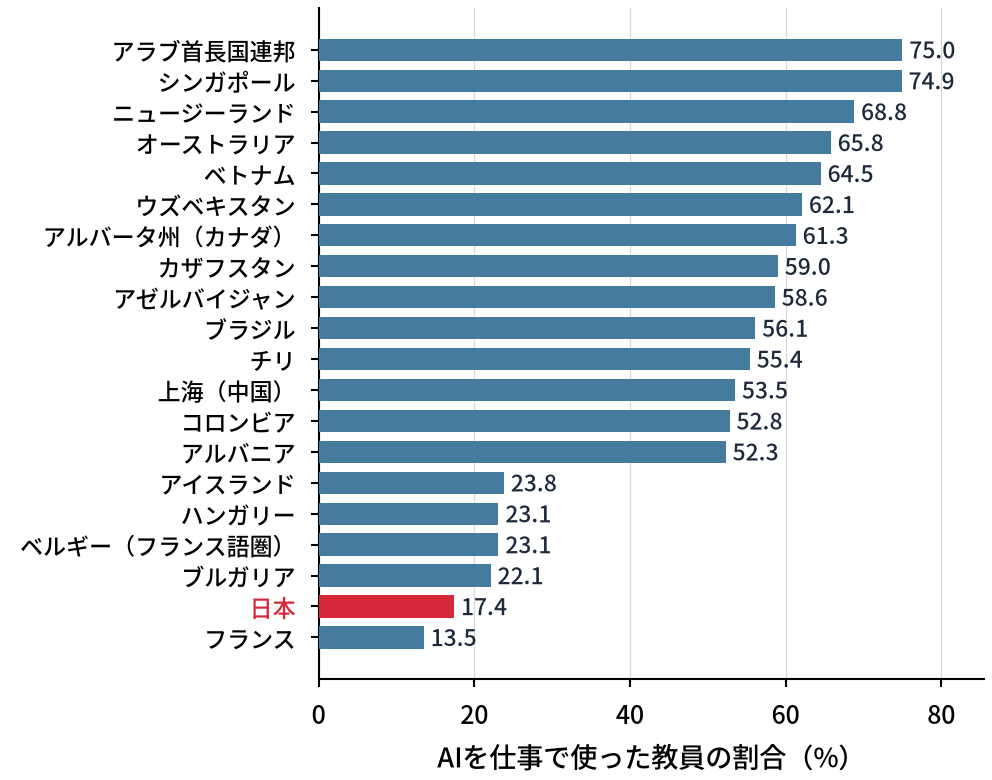
\includegraphics[width=\columnwidth]{chart_oecd_talis_teacher_survey.png}\caption{AIを仕事で使った教員の割合の値の比較（上位・下位と日本を抜粋）}\end{figure}
\begin{figure}[t]\centering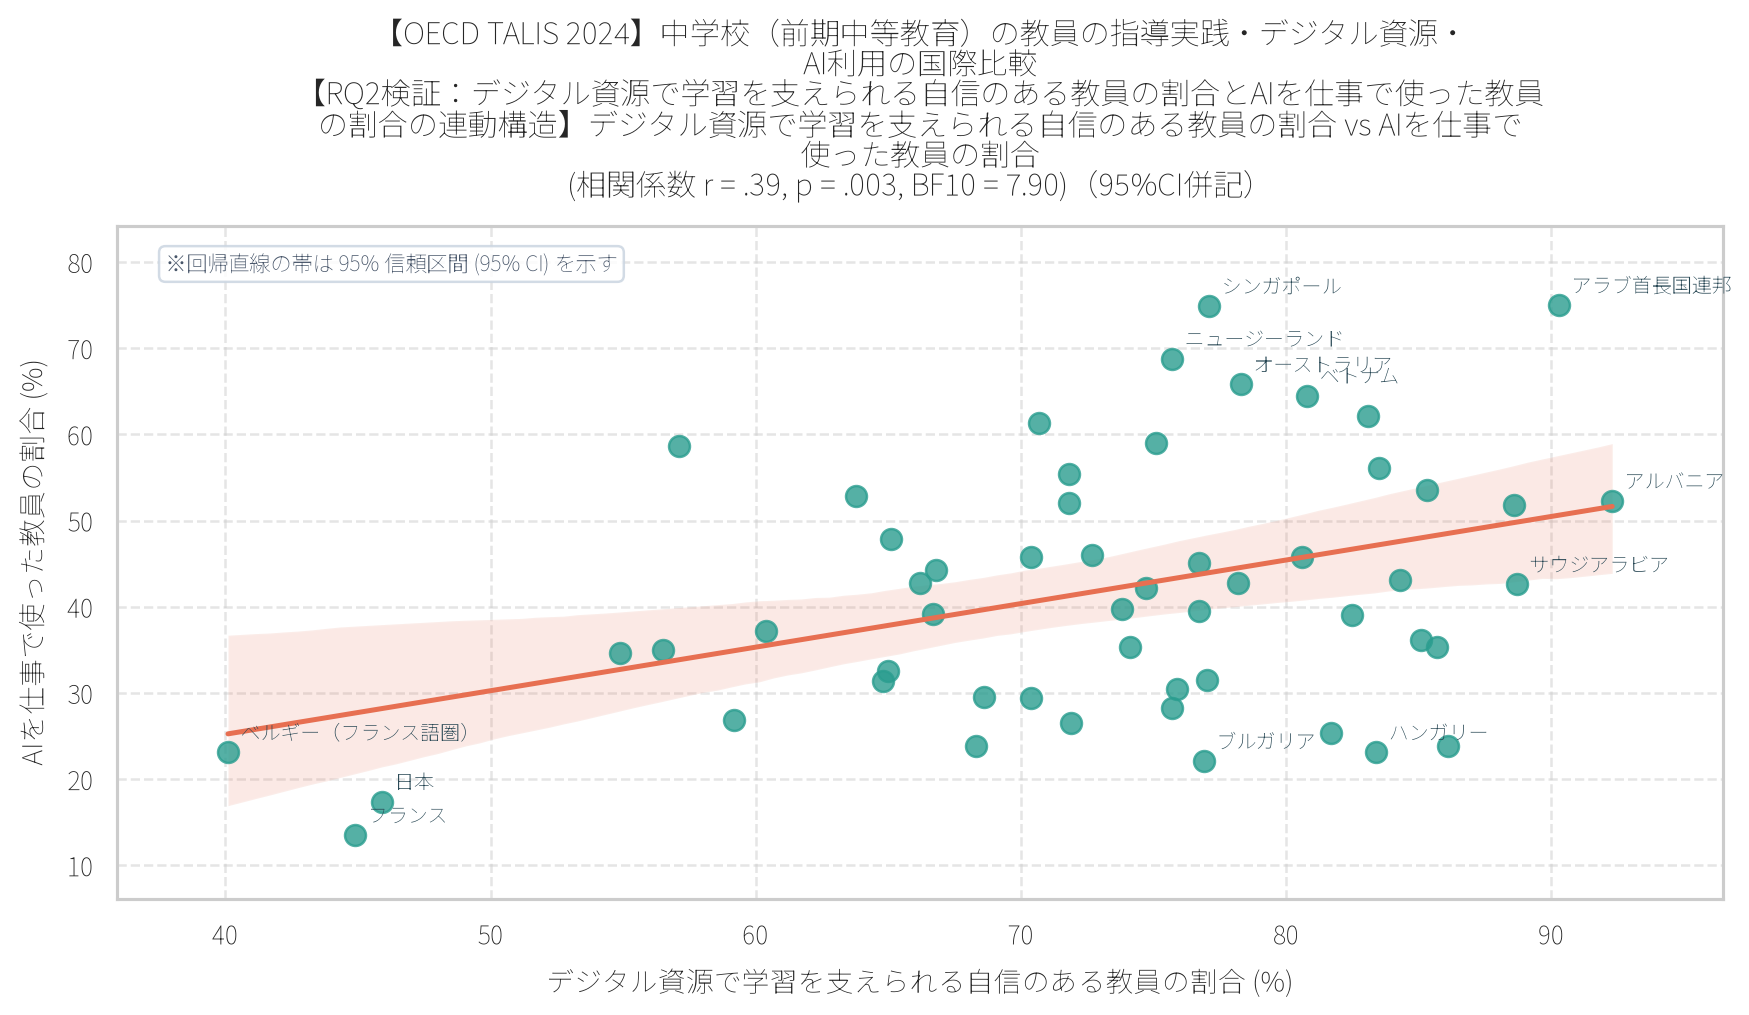
\includegraphics[width=\columnwidth]{chart_secondary_oecd_talis_teacher_survey.png}\caption{デジタル資源で学習を支えられる自信のある教員の割合とAIを仕事で使った教員の割合の関連（回帰直線と95\%信頼区間の帯）}\end{figure}
\section{考察}
RQ1とRQ2の結果をまとめると，日本の中学校の教員は，デジタル資源を使わせる割合，その自信，AIの利用のいずれも54の国・地域のなかで低い位置にあり，とくにAIの利用と自信は下から2番目と3番目であった．これはOECD (2025)の表の範囲で確かめられることで，27か国のOECD平均と54の国・地域の単純平均（AI 41.88\%，自信73.0\%）のどちらと比べても変わらない．ただし，この低さを教員の力量や意欲の低さと読むことはできない．OECD (2020)と国立教育政策研究所 (2019)は，2018年の調査を報告しているが，本稿は同じ質問での変化を確かめていない．

自信とAIの利用の正の関連は，教員の技術活用に自信が関わるとするErtmer and Ottenbreit-Leftwich (2010)の議論と，向きとしては矛盾しない．しかし，この議論は個々の教員についてのものであり，国・地域の集計値の関連から，自信のある教員ほどAIを使うとは言えない（生態学的誤謬）．また，AIの利用は少人数グループの指導とも同程度以上に関連しており（\textit{r}=.59），デジタル資源への自信に固有の関連とは言えない．新しい取り組みに肯定的に答える傾向が国・地域によって異なり，複数の指標に共通して表れている可能性が考えられるが，これが回答の仕方の違いなのか，実際の取り組みの違いなのか，あるいは経済水準や学校のICT環境，国・地域のまとまりによる偏りなのかは，本研究のデータでは区別できない．

Rogers (2003)の枠組みに照らせば，AIの利用の違いは普及の程度の違いとして読めるが，1時点のデータでは過程を追えない．Fullan (2016)や佐藤 (2012)が学校全体の変化を論じ，Vangrieken et al. (2015)が教員の協働を整理したことを踏まえると，新しい道具の利用には学校の取り組みや教員どうしの関係も関わる可能性があるが，仮説にとどまる．Vieluf et al. (2012)はTALISから指導実践を論じたが，日本の批判的思考を要する課題の割合（24.2\%）の低さも，同じ慎重さで読む必要がある．

校内でデジタル資源やAIの使い方を共有する機会をつくることは一つの方向として考えられるが，その効果は確かめられていない．本研究の限界は，(1)集計値のみで個人の因果を特定できないこと，(2)自己申告であること，(3)4つの国・地域に無回答による偏りの注意があること，(4)経済水準やICT環境を統制していないこと，(5)1時点のデータであること，(6)全ペアの探索で多重比較の影響を受けうること，である．
\section*{参考文献}
\begingroup\scriptsize\setlength{\parindent}{0pt}\raggedright
\par\hangindent=1.5\zw\hangafter=1 ERTMER, P. A. and OTTENBREIT-LEFTWICH, A. T. (2010) Teacher technology change: How knowledge, confidence, beliefs, and culture intersect. Journal of Research on Technology in Education, \textbf{42} (3) ：255-284.\vspace{1pt}
\par\hangindent=1.5\zw\hangafter=1 FULLAN, M. (2016) The New Meaning of Educational Change. Teachers College Press.\vspace{1pt}
\par\hangindent=1.5\zw\hangafter=1 国立教育政策研究所 (2019) 教員環境の国際比較：OECD国際教員指導環境調査（TALIS）2018報告書―学び続ける教員と校長―. ぎょうせい.\vspace{1pt}
\par\hangindent=1.5\zw\hangafter=1 OECD (2020) TALIS 2018 Results (Volume II): Teachers and School Leaders as Valued Professionals. OECD Publishing, Paris. DOI: 10.1787/19cf08df-en\vspace{1pt}
\par\hangindent=1.5\zw\hangafter=1 OECD (2025) Results from TALIS 2024: The State of Teaching. OECD Publishing, Paris. DOI: 10.1787/90df6235-en\vspace{1pt}
\par\hangindent=1.5\zw\hangafter=1 ROGERS, E. M. (2003) Diffusion of innovations (5th ed.). Free Press.\vspace{1pt}
\par\hangindent=1.5\zw\hangafter=1 佐藤学 (2012) 学校を改革する：学びの共同体の構想と実践. 岩波書店.\vspace{1pt}
\par\hangindent=1.5\zw\hangafter=1 VANGRIEKEN, K., DOCHY, F., RAES, E. and KYNDT, E. (2015) Teacher collaboration: A systematic review. Educational Research Review, \textbf{15} ：17-40.\vspace{1pt}
\par\hangindent=1.5\zw\hangafter=1 VIELUF, S., KAPLAN, D., KLIEME, E. and BAYER, S. (2012) Teaching Practices and Pedagogical Innovations: Evidence from TALIS. OECD Publishing, Paris. DOI: 10.1787/9789264123540-en\vspace{1pt}
\endgroup
\section*{Summary}
{\footnotesize\setlength{\parindent}{0pt}Using the published TALIS 2024 tables, we described, for lower secondary teachers in 54 countries and economies, the share of teachers who let students use digital resources, the share who feel confident in supporting student learning with digital resources, and the share who used AI for their work in the 12 months before the survey. In Japan, 17.4\% of teachers had used AI for work (OECD average 36.3\%), ranking 53rd of 54, and 45.9\% were confident in supporting learning with digital resources (OECD average 70.1\%), ranking 52nd. Across countries, the share of confident teachers and the share of teachers using AI were weakly to moderately and positively correlated (r = .39, BF10 = 7.9). However, AI use was at least as strongly related to the share of teachers who ask students to work in small groups on joint solutions (r = .59), so the association is not specific to digital confidence. These are associations between self-reported country-level aggregates and do not show causation in the behaviour of individual teachers.\par\smallskip KEYWORDS: TALIS 2024, TEACHERS, DIGITAL RESOURCES, ARTIFICIAL INTELLIGENCE, CROSS-COUNTRY\par}
\medskip\noindent\fbox{\parbox{\dimexpr\columnwidth-2\fboxsep-2\fboxrule}{\footnotesize\gtfamily 【付記：生成AIによる自動執筆に関する開示】\\ 本論文は学生への教育目的で作成している．使用しているデータは公的オープンデータである．統計の算出はPythonで行い，文章は生成AI（Anthropic Claude等）を活用して作成した．記載した統計数値は元データに準拠しているが，教育学的な考察や提言の妥当性は，指導現場の実情に応じて，批判的に吟味してほしい．}}
\end{document}
